\documentclass[a0paper,portrait]{baposter}

\usepackage{lipsum}          % This is just for some blindtext
\usepackage{biblatex}
\usepackage{relsize}	       % For \smaller
\usepackage{url}			       % For \url
\usepackage{epstopdf}	       % Included EPS files automatically converted to PDF to include with pdflatex
\usepackage{multicol}        % Multi Columns

\usepackage{amsmath} % math
\usepackage{amssymb}
\usepackage{accents}
\usepackage[slovak]{babel}
\usepackage{csquotes}
\usepackage{xcolor}
\usepackage{marvosym}


%%%%%%%%%%%%%%%%%%%%%%%%%%%%%%%%%%%%%%%%%%%%%%%%%%%%%%%%%%%%%%%%%%%%%%%%%%%%%%%%
%%% Utility functions %%%%%%%%%%%%%%%%%%%%%%%%%%%%%%%%%%%%%%%%%%%%%%%%%%%%%%%%%%
%%%%%%%%%%%%%%%%%%%%%%%%%%%%%%%%%%%%%%%%%%%%%%%%%%%%%%%%%%%%%%%%%%%%%%%%%%%%%%%%

%%% Save space in lists. Use this after the opening of the list %%%%%%%%%%%%%%%%
\renewcommand{\vec}[1]{\bm{#1}}
%\renewcommand{\dot}[1]{\accentset{\cdot}{#1}}
\renewcommand{\ddot}[1]{\stackrel{..}{#1}}
%\newcommand{\tildeI}[1]{\overset{\tilde{}}{#1}} 

%\renewcommand{\bibname}{}

\newcommand{\vnabla}{\vec{\nabla}}

\renewcommand{\d}[1]{\text{d} #1}
\newcommand{\dxx}{\,\text{d}\vec{x}}
\newcommand{\dx}{\,\text{d}x}

\newcommand{\diff}[2]{\frac{\text{d}#1}{\text{d}#2}}
\newcommand{\idiff}[2]{\text{d}#1 / \text{d}#2}
\newcommand{\pdiff}[2]{\frac{\partial #1}{\partial #2}}
\newcommand{\pdifff}[2]{\frac{\partial^2 #1}{\partial #2^2}}
\newcommand{\ipdiff}[2]{\partial #1 / \partial #2}
\newcommand{\vdiff}[2]{\frac{\delta #1}{\delta #2}}
\newcommand{\ivdiff}[2]{\delta #1 / \delta #2}

\definecolor{mcr_purple}{RGB}{108,44,145}

%%%%%%%%%%%%%%%%%%%%%%%%%%%%%%%%%%%%%%%%%%%%%%%%%%%%%%%%%%%%%%%%%%%%%%%%%%%%%%%
%%% Document Start %%%%%%%%%%%%%%%%%%%%%%%%%%%%%%%%%%%%%%%%%%%%%%%%%%%%%%%%%%%%
%%%%%%%%%%%%%%%%%%%%%%%%%%%%%%%%%%%%%%%%%%%%%%%%%%%%%%%%%%%%%%%%%%%%%%%%%%%%%%%

\begin{document}
\typeout{Poster rendering started}

%%% General Poster Settings %%%%%%%%%%%%%%%%%%%%%%%%%%%%%%%%%%%%%%%%%%%%%%%%%%%
%%%%%% Eye Catcher, Title, Authors and University Images %%%%%%%%%%%%%%%%%%%%%%
\begin{poster}{
  columns=2,
	grid=false,
	borderColor=uniblue,
	headerColorOne=uniblue,
	headerColorTwo=uniblue,
	headerFontColor=white,
  headerheight=14em,
	boxColorOne=white,
  boxpadding=1em,
	headershape=rounded,
	headerfont=\Large\textsf,
	textborder=rounded,
	background=shadetb,
  bgColorOne=uniblue!10,
  bgColorTwo=uniblue!30,
	headerborder=open,
  boxshade=plain,
  eyecatcher=false
}
%%% Eye Cacther %%%%%%%%%%%%%%%%%%%%%%%%%%%%%%%%%%%%%%%%%%%%%%%%%%%%%%%%%%%%%%%
{ %\vspace{1em}
}
%%% Title %%%%%%%%%%%%%%%%%%%%%%%%%%%%%%%%%%%%%%%%%%%%%%%%%%%%%%%%%%%%%%%%%%%%%
{\vspace{1.25em} 
\smaller How long does it take for a cup of coffee to cool down?}
%%% Authors %%%%%%%%%%%%%%%%%%%%%%%%%%%%%%%%%%%%%%%%%%%%%%%%%%%%%%%%%%%%%%%%%%%
{
  \vspace{1.5em}
  {  \textbf{General Physics Group 55} \\
	{\smaller Diyaco Shwany, Jakub \v{S}\v{t}avina, Tomas Kvietkauskas, Phartav Murukutla, Aidan Hall, Jac Evans \\ 
    \textcolor{mcr_purple}{\smaller Department of Physics and Astronomy, University of Manchester}
    }
}
}
%%% Logo %%%%%%%%%%%%%%%%%%%%%%%%%%%%%%%%%%%%%%%%%%%%%%%%%%%%%%%%%%%%%%%%%%%%%%
{\begin{minipage}{18.0em}
    
\includegraphics[height=7.5em]{logo-uni.pdf}
  \end{minipage}}

%%% Abstract %%%%%%%%%%%%%%%%%%%%%%%%%%%%%%%%%%%%%%%%%%%%%%%%%%%%%%%%%%%%%%%%%%
\headerbox{Abstract}{name=abstract,column=0,row=0,span=2}{
%\begin{multicols}{2} 
    Lorem ipsum dolor sit amet, consectetur adipiscing elit, sed do eiusmod tempor incididunt ut labore et dolore magna aliqua. Ut enim ad minim veniam, quis nostrud exercitation ullamco laboris nisi ut aliquip ex ea commodo consequat. Duis aute irure dolor in reprehenderit in voluptate velit esse cillum dolore eu fugiat nulla pariatur. Excepteur sint occaecat cupidatat non proident, sunt in culpa qui officia deserunt mollit anim id est laborum.

%\end{multicols}
}

%%% Box 1 %%%%%%%%%%%%%%%%%%%%%%%%%%%%%%%%%%%%%%%%%%%%%%%%%%%%%%%%%%%%%%%%%%%%%
\headerbox{Introduction}{name=box1,column=0,below=abstract%,above=bottom
}{As physics students, we often find ourselves in dire need of a productivity boost in the form of a cup of coffee. However, as most time is spent on physics, it is easy to be too eager to drink the coffee too soon or forget it so it goes cold. We aim to provide struggling students with an understanding of the temperature depenence on time of a cup of coffee left at room temperature.
%First, we performed a simple experiment and fit an empirical model based on Newton's law of cooling. To understand the underlying physics better, we then constructed a theoretical model of the heat equation on a rectangular cup of coffee.
 
  %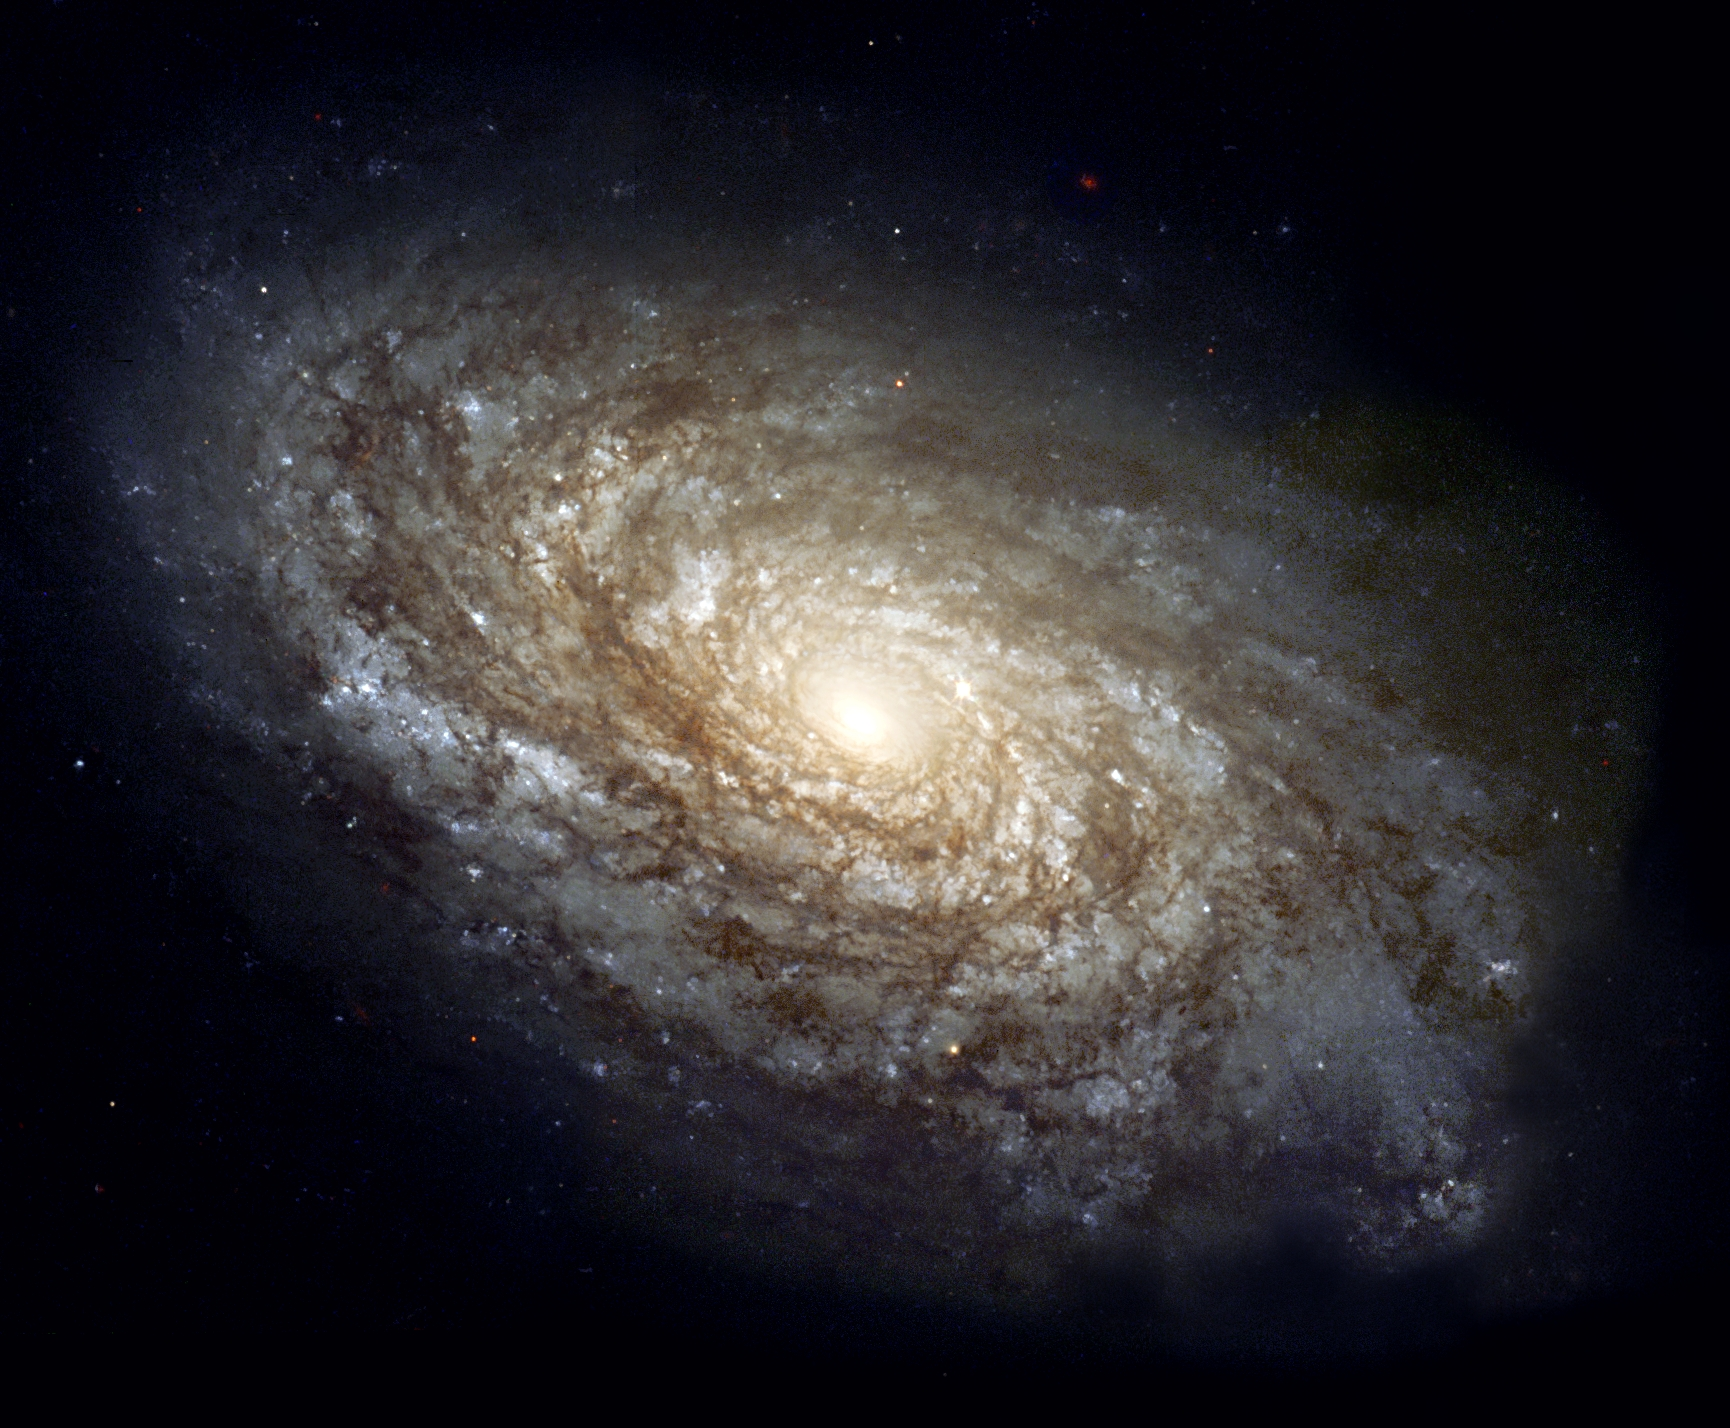
\includegraphics[width=\textwidth]{figure_1.jpg}
  %\caption{This is my caption.}
}

\headerbox{Theory}{name=model_0,column=0,below=box1%,above=bottom
}{Excepteur sint occaecat cupidatat non proident, sunt in culpa qui officia deserunt mollit anim id est laborum.
Excepteur sint occaecat cupidatat non proident, sunt in culpa qui officia deserunt mollit anim id est laborum.
Excepteur sint occaecat cupidatat non proident, sunt in culpa qui officia deserunt mollit anim id est laborum.
Excepteur sint occaecat cupidatat non proident, sunt in culpa qui officia deserunt mollit anim id est laborum.
Excepteur sint occaecat cupidatat non proident, sunt in culpa qui officia deserunt mollit anim id est laborum.
}

%%%%%%%%%%%%%%%%%%%%%%%%%%%%%%%%%%%%%%%%%%%%%%%%%%%%%%%%

\headerbox{Empirical Model}{name=model_1,column=0,below=model_0%,above=bottom
}{Using a digital probe thermometer, we measured the temperature of a cup of hot coffee over time, as shown in Figure ?, at room temperature of 17°C. The starting temperature of the coffee ranged between 85 - 90°C.

Using Newton's law of cooling,

\begin{equation}
    \frac{dQ_{coffee}}{dt} = h_{air}A_{top}(T_{surr} - T_{coffee}) + h_{cup}A_{inner}(T_{cup} - T_{coffee})
\end{equation}
    
\begin{equation}
    \frac{dQ_{cup}}{dt} = h_{air} A_{outer}(T_{surroundings} - T_{cup}) + h_{cup}A_{inner}(T_{coffee} - T_{cup})
\end{equation}
assuming the transfer coefficient from the cup to the air is the same as that from the coffee to the air. Here the values $h_{air}$ and $h_{cup}$ are left to be determined empirically. To solve these equations numerically, we performed a time-stepping procedure $\delta Q (t' + \delta t) = \frac{dQ}{dt} \Bigr|_{t = t'} \delta t$. We could then calculate the temperature change $\delta T$ Using the specific heat capacity $c$ of each material of mass $m$, we have $\delta T (t' + \delta t) = \delta Q(t' + \delta t')/cm$.

The model was then fitted to the empirical data, as shown in Figure ?. This yielded the values of the heat transfer coefficients of $h_{air} \approx 27.8$ $ Wm^{-2}K^{-1}$, $h_{cup} \approx 26.3 $ $Wm^{-2}K^{-1}$. The lower heat transfer coefficient of the cup relative to the air demonstrates that it acts as insulation for the cooling coffee.

}


%%% Box 2 %%%%%%%%%%%%%%%%%%%%%%%%%%%%%%%%%%%%%%%%%%%%%%%%%%%%%%%%%%%%%%%%%%%%%
\headerbox{Theoretical Model}{name=model_2,column=1,below=abstract%,above=bottom
}{
 We assumed that the dominant form of cooling was due to convection by the air and used the heat equation to describe the coffee itself. The convective cooling was incorporated into the system as boundary conditions, and we expected the sides and bottom of the cup to be more insulated than the open surface at the top. The form of the boundary condition was motivated using Newton’s law of cooling. To simplify calculations, we assumed the cup was a cuboid. The aim was to numerically solve the 3D heat equation, 

\begin{equation}
    \frac{\partial^2 T }{\partial t^2} = \alpha \left( \frac{\partial^2 T }{\partial x^2} + \frac{\partial^2 T }{\partial y^2} + \frac{\partial^2 T }{\partial z^2} \right)
\end{equation}

Using the following robin boundary conditions, 

\begin{equation}
    \frac{\partial T}{\partial z} \Bigr|_{z = 0} = - \frac{h_{cup}}{k_{water}} (T - T_{\infty})
\end{equation}

\begin{equation}
    \frac{\partial T}{\partial z} \Bigr|_{z = H} = - \frac{h_{air}}{k_{water}} (T - T_{\infty})
\end{equation}

where $H$ is the height of the cup and $k_{water}$ is the thermal conductivity of water. The conditions in other coordinates were identical but all featured $h_{cup}$, as only the top of the cup is exposed to air. The empirical model values for $h_{cup}$ and $h_{air}$ were used.

The solution method was an explicit FDM scheme which discretises the system. In 1D the scheme creates the following map,

\begin{equation}
    T_i^{n+1} = T_i^n + \frac{\alpha \delta t}{(\delta x)^2} (T_{i-1}^{n} - 2 T_i^n + T^n_{i+1})
\end{equation}

Where the 3D generalisation is straightforward. The scheme is first order consistent. The forward Euler scheme was used to integrate the boundary conditions only across the outer walls of the 3D discretised system. The corners and edges of each face was ignored in the simulation as the scheme being used never updates those cells. \\
The plot of temperature against time was found by averaging the temperature of only the inner nodes of the discretised system. The walls were ignored in the average as they introduced an unphysical drop in the temperature after the initial time step. However, this plot abstracts the temperature distribution which never fully became uniform in the simulation.


%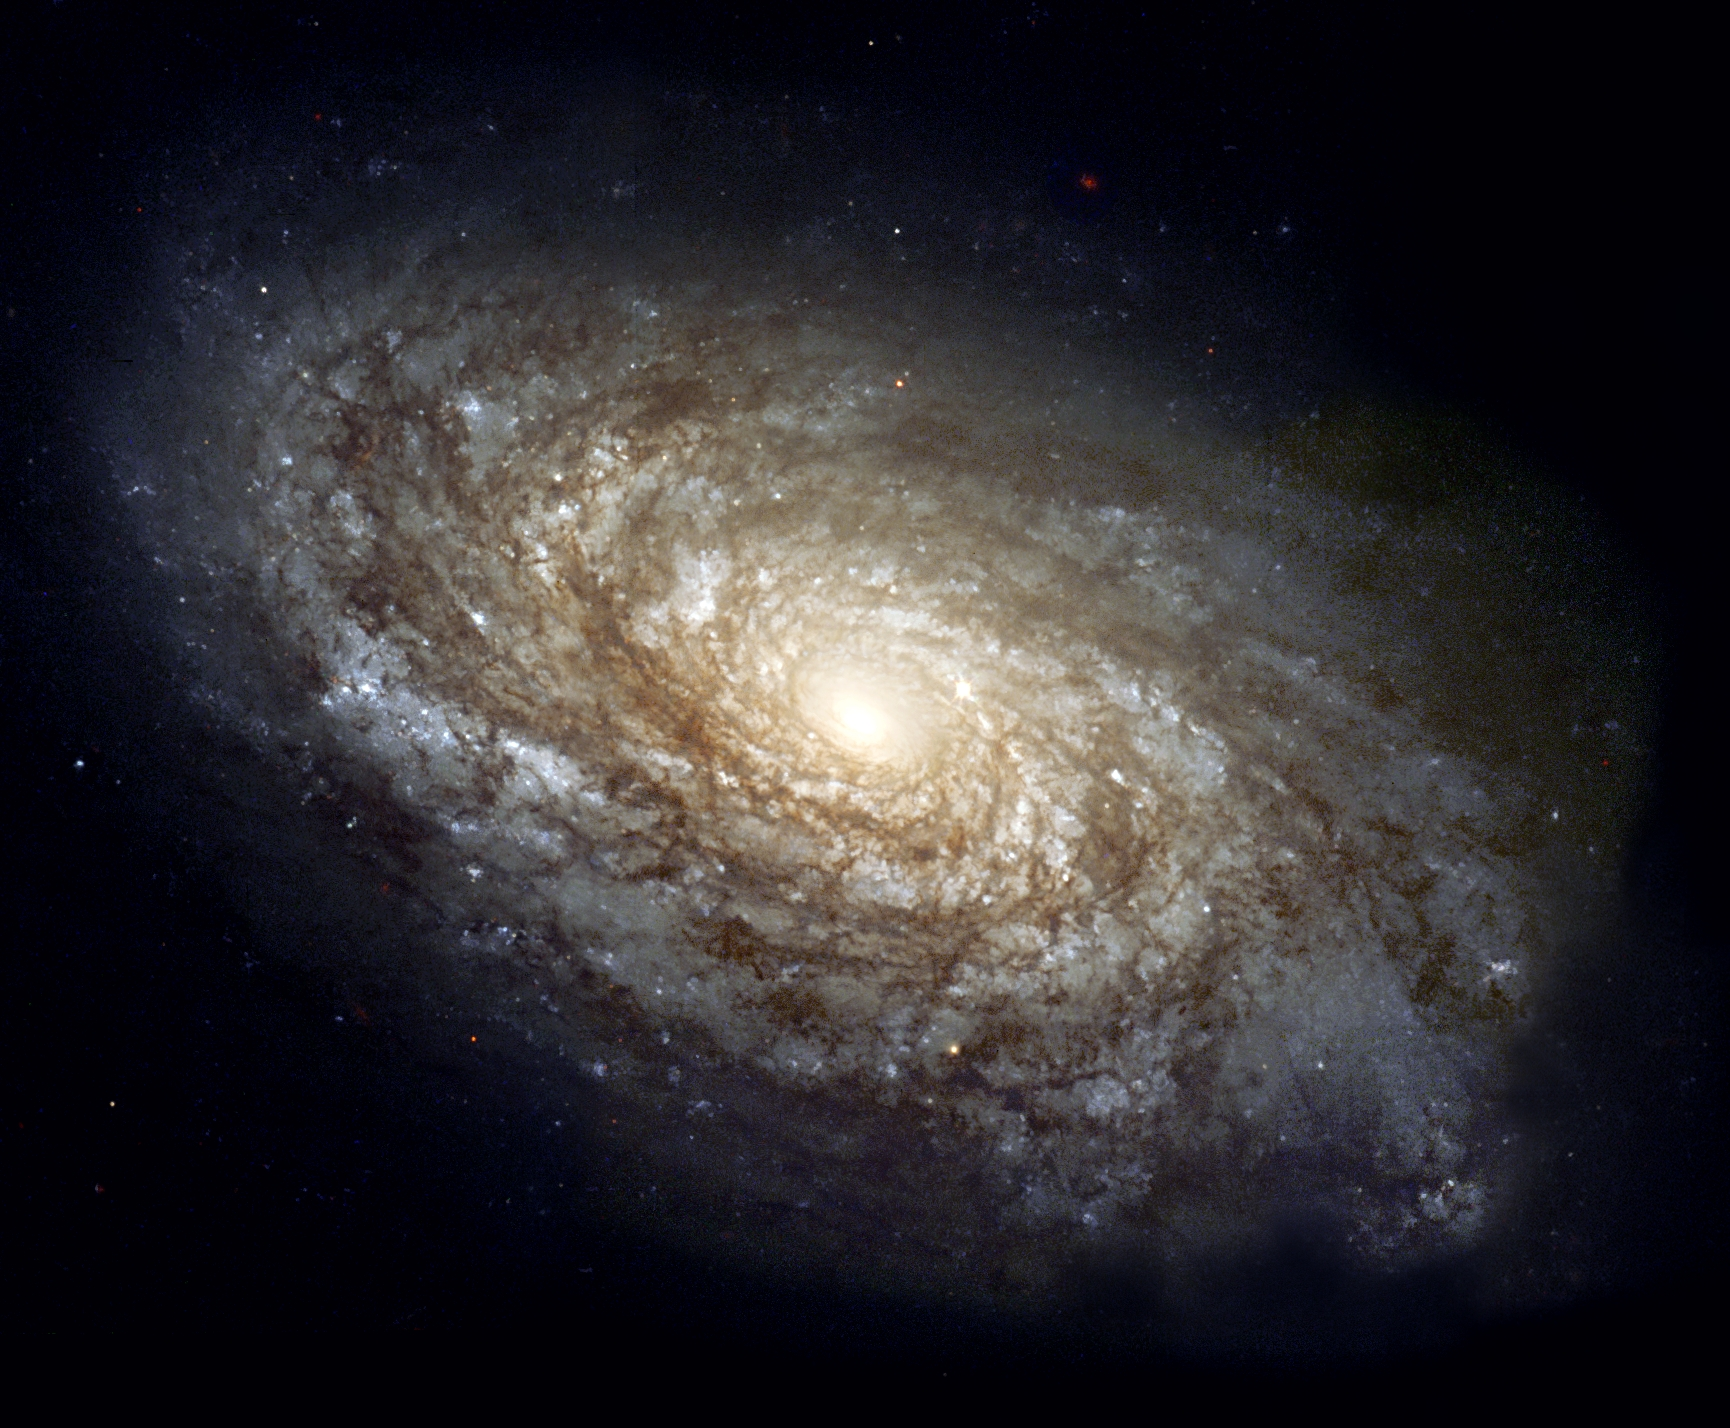
\includegraphics[width=\textwidth]{figure_1.jpg}

} 

\headerbox{Discussion}{name=conclusions,column=1,below=model_2}{  
%\begin{figure}[t]
%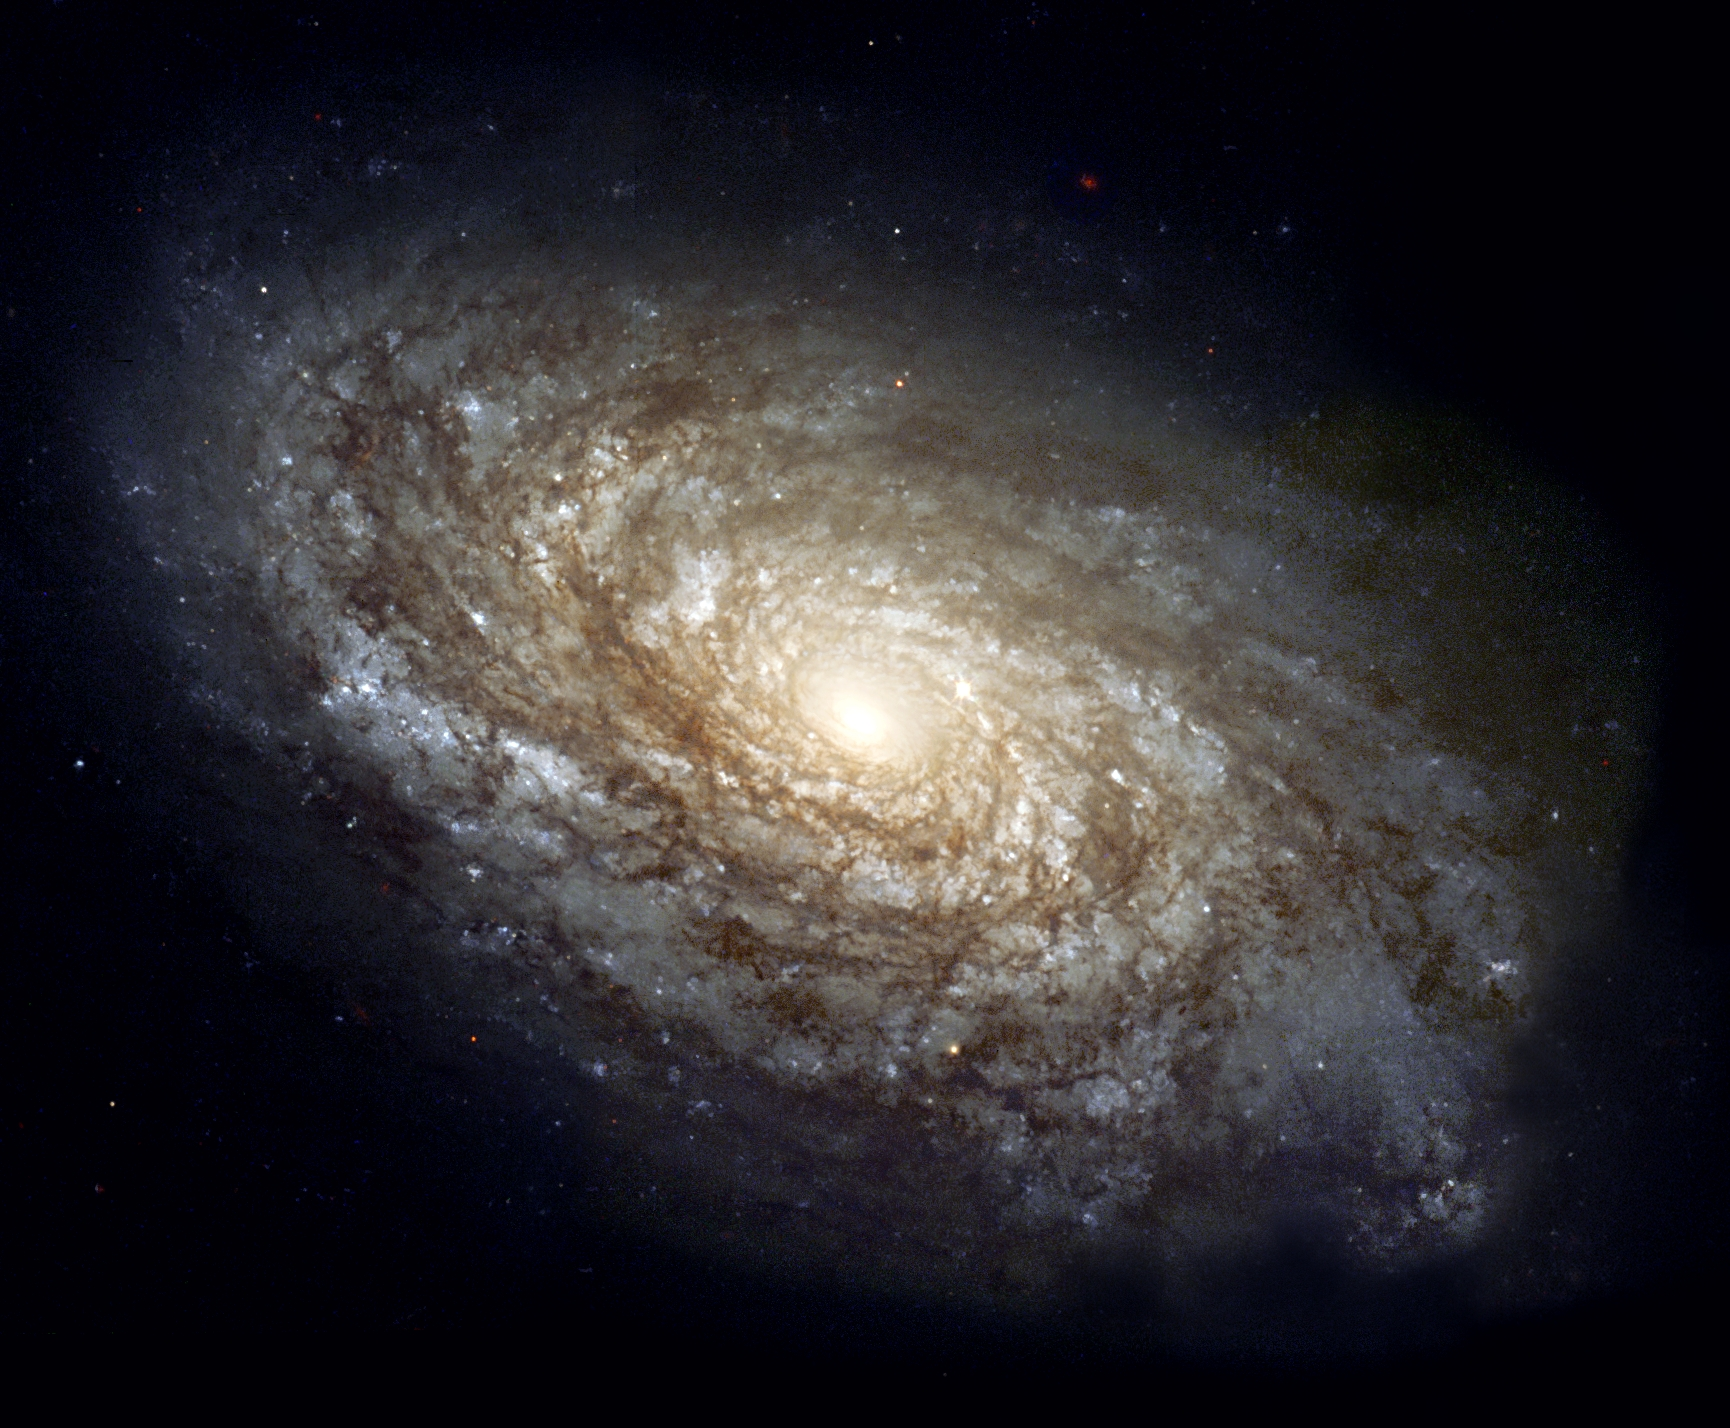
\includegraphics[width=0.5\textwidth]{figure_1.jpg}
%\caption{This is my caption.}
%\end{figure}

The theoretical model predicts that the coffee cools slower compared to the experimental data. This was to be expected as the heat equation assumes that heat can only spread throughout the coffee due to diffusion. A real fluid would have convective mixing which would allow the heat to disperse much faster. Furthermore, the boundary condition ignores evaporative cooling. Evaporative cooling would likely cause the initial drop in temperature to be a lot faster, but its effect would diminish as the coffee cools down. These contributions form the basis of next steps to improve the accuracy of the model. It would also be informative to use higher order FDM schemes as a consistency check. 

}

\headerbox{References}{name=references,column=0,below=conclusions, span=2}{

\renewcommand{\section}[2]{}
\begin{thebibliography}{9}
\bibitem{Topinka2001} M. A. Topinka, B. J. LeRoy, R. M. Westervelt, S. E. J. Shaw, R. Fleischmann, E. J. Heller, K. D. Maranowski, and A. C.
Gossard, Nature (London) {\bf 410}, 183 (2001).
\bibitem{Patsyk2020} A. Patsyk, U. Sivan, M. Segev, and M. A. Bandres, Nature
(London) {\bf 583}, 60 (2020).
\bibitem{Kaplan2002} L. Kaplan, Phys. Rev. Lett. {\bf 89}, 184103 (2002).
\end{thebibliography}

}

\end{poster}
\end{document}
